
See Appendix \ref{cilkAppendix} for history and background of cilk.

\subsection{Cilk Implementation: Recursive}

The classic Cooley-Tukey FFT algorithm makes use of recursion to reduce computation time of FFT decomposition by splitting up the even and odd terms. Cilk parallelism can be exposed in recursive algorithms with ease by utilizing the \texttt{cilk\_spawn} and \texttt{cilk\_sync} keywords. Since the even and odd terms of the FFT are independent a CPU with sufficient resources will be able to compute these in parallel given cilk’s spawn routines. When both spawned children are done they must be synced to ensure coherent programming order.

From a programming point of view, cilk is a very easy tool for the programmer to use since the recursive routine can first be written without any cilk constructs. When functional correctness is established, the cilk keywords may be introduced.

The merging step that occurs after the divide and conquer steps are complete can also expose parallelism to cilk. In our implementation this step is called via the \texttt{cilk\_combine()} function. Cilk spawns two threads of \texttt{cilk\_combine()} with arrays of half the size. When the sub-arrays reach below a certain threshold of \texttt{cilk\_max\_recombine}, the \texttt{cilky\_combine()} function is called. This function uses the \texttt{cilk\_for} construct to parallelize work.

From a parallel algorithms perspective it is interesting to note the performance impact of the value of \texttt{cilk\_max\_recombine}. Figure \ref{cilk_max_recombine} shows that as the number of elements of the FFT grows, there is a noticeable performance gap between the two cilk recursive runs where the only change is in the value of \texttt{cilk\_max\_recombine} (value of 1 vs. 128). A value of 128 represents fewer threads processing more values in \texttt{cilky\_combine()} as compared to a value of 1 where more threads are processing fewer elements in parallel. This is akin to the cascaded parallel algorithm technique of splitting up the groups of elements a certain way to achieve a work-optimal solution. 

It should be noted that the recursive solution is still of work-complexity $\mathcal{O}(n * log(n))$ as the algorithm is not changed. However, the cilk constructs expose potential parallelism which means that overall running time is decreased given system resources. 



\subsection{Cilk Implementation: Iterative}
The introduction of the \texttt{cilk\_for} construct allows for loops with independent operations to run in parallel. Replacing one \texttt{for} with a \texttt{cilk\_for} in the \texttt{cilk\_transform\_iter()} function results in a dramatic performance boost as can be seen in the graph of figure \ref{iterative_fft}. 
Similarly to the recursive cilk implementation, the cilk iterative algorithm is still of the same complexity, $W(n) = \mathcal{O}(n * log(n))$, but is faster due to the exposed parallelism. 

\subsection{Cilk Analysis}
As can be seen in the graph of figure \ref{fft_cilk_cpp}, the performance differences between the five different algorithms becomes clear when processing at least 2\textsuperscript{10} elements. The non-cilk C++ recursive algorithm is the slowest performance-wise. The recursive recursive  implementation that uses a value of \texttt{cilk\_max\_recombine} value of 1 is faster than the non-cilk version, but not by much. An interesting observation is that the cilk recursive algorithm with a \texttt{cilk\_max\_recombine} value of 128 is faster than the version that uses a value of 1 for all values save some outliers. In fact, it is close to \( \frac{2}{3} \) the completion time of the \texttt{cilk\_max\_combine} value of 1.

\begin{figure}
\center
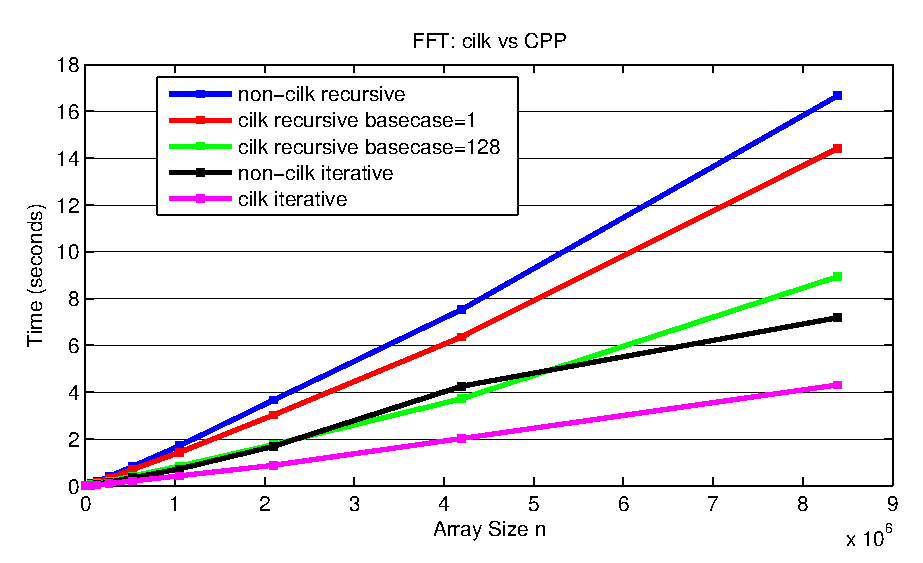
\includegraphics[scale=0.8]{img/fft_cilk_cpp.eps}
\caption{Graph comparing the performance of all FFT algorithms, cilk and C++} 
\label{fft_cilk_cpp}
\end{figure}

Moreover, the iterative cilk implementation is by far the highest performing algorithm. It is about 1.6x times faster than the non-cilk version for large values. Another observation worth noting is that the iterative non-cilk solution is ~2.3x faster than its non-cilk version. This relationship is similar between the cilk iterative implementation and the recursive cilk \texttt{cilk\_max\_recombine}=128 solution (~2x performance gains), while it grows to as much as ~3.3x as compared to the recursive cilk \texttt{cilk\_max\_recombine}=1 solution . 

Cilk does provide built-in ways to adjust the “grain-size” of the threads. This was not used in this project; however, from the curves of the graph in figure \ref{cilk_max_recombine} it is obvious that a lot of performance improvement can be gained with calibration of the number of threads cilk uses. 

The parallelism gained by cilk comes at the cost of memory (space complexity) usage. Inherently, it is very difficult to measure stack usage by cilk since it manipulates the stack so much to achieve parallelism that any attempts to trace stack usage affects cilk performance negatively. However, heap usage is easy to measure using the program profiling tool Valgrind with the heap profiler massiff. As can be seen from images in figure \ref{fig:masiff}, the iterative cilk solution that uses the \texttt{cilk\_for} construct does not use much more heap space than the non-cilk iterative one. This may be due to cilk’s internal vectorization instead of the spawn/sync mechanism. The recursive cilk solution uses more heap space than the non-cilk version (~41MB vs. ~28MB). 

